\documentclass[12pt]{article}
\usepackage{amsmath}  % Math
\usepackage{amssymb}  % Symbols
\usepackage{graphicx} % Images
\usepackage[utf8]{inputenc}
\usepackage[T1]{fontenc}
\usepackage[margin=1in]{geometry}
\usepackage[spanish]{babel}
\usepackage{transparent}
\usepackage{eso-pic}
\usepackage{xcolor}

\graphicspath{{images/}} % Path to images
\newcommand\BackgroundPic{
    \put(0,0){
        \parbox[b][\paperheight]{\paperwidth}{
            \vfill
            \centering
            \transparent{0.2}
\includegraphics[width=\paperwidth]{logo} % your image
            \vfill
        }
    }
}


\title{Informe Negocio Empanadas: \\
  \textit{Empanadas de Juancho, 100\% Legales}}
  \author{Autores: Felipe Colli, Juan Gonzalez, Bastián Ortiz y Javier Robles \thanks{Instituto Nacional General José Miguel Carrera} \\ Curso: \textit{4°H}, Profesor: \textit{Carlos Morales}} % Add your names and course
\date{\today}
\AddToShipoutPicture{\BackgroundPic} % Add background image

\begin{document}

\maketitle
%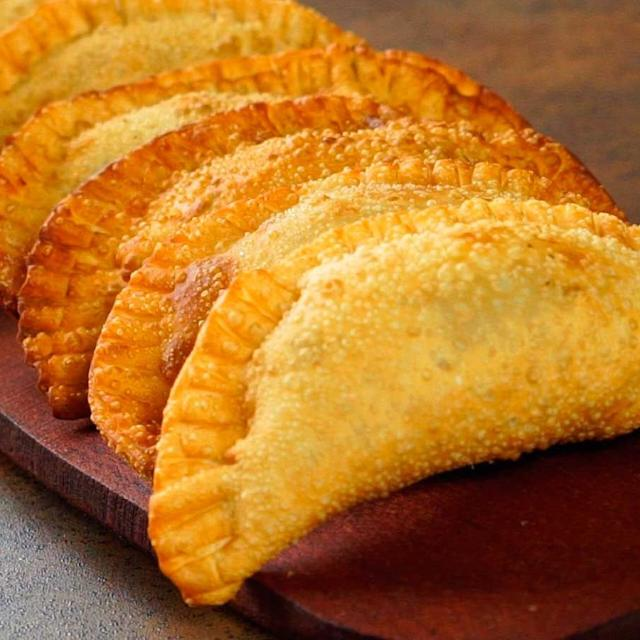
\includegraphics[width=0.95\textwidth]{empanadas} % Logo of the school
\newpage

\tableofcontents
\newpage

\section{Resumen} % Aprox 1/3 de Pagina

\newpage



\section{Introducción} % Max 1 pagina
El presente informe tiene como objetivo presentar el negocio de empanadas "Empanadas de Juancho", un emprendimiento que busca ofrecer empanadas de alta calidad. A través de este documento, se detallarán los aspectos clave del negocio, incluyendo su propuesta de valor, mercado objetivo y proyecciones financieras. \\


Dentro de las proyeciones financieras, se contempla un análisis de costos y precios, así como una estimación de las ganancias esperadas. El negocio se enfoca en la producción y venta de 3 variedades de empanadas, con un énfasis en la calidad de los ingredientes y la satisfacción del cliente, sin olvidar el marco legal regulatorio, por lo cual este negocio no sera un frente para lavado de activos, evasion de impuestos, generacion de facturas ideologicamnete falsas, o la venta de drogas. \\ % Referencia a Brekain Bad y Los Pollos Hermanos 


Otro objetivo clave de este informe es proporcionar un analisis detallado de la viabilidad del negocio, incluyendo un estudio de mercado que identifique las oportunidades y desafíos en el sector de alimentos. Se espera que este informe sirva como una guía para la implementación exitosa del negocio y como una herramienta para atraer posibles inversores interesados en el proyecto.
\newpage



\section{Desarrollo} % 2 - 5 paginas

\subsection{Tabla de Costos Ingredientes}

\begin{table}[h!]
    \centering
    \begin{tabular}{|| c | c | c | c | c||} %MAsa Prehecha || costo en Negocio 1 || costo por unidad en Negocio 1 || costo en Negocio 2 || costo por unidad en Negocio 2
        \hline
        \textbf{Masa} & \textbf{C Negocio 1} & \textbf{C/U Negocio 1} & \textbf{C Negocio 2} & \textbf{C/U Negocio 2} \\ [0.5ex]
        \hline\hline

        \multicolumn{5}{||c||}{\textbf{Masa Prehecha de Queso Chica}} \\ [0.5ex] \hline \hline
        Masa 1 & \$1000 & \$1000 & \$1200 & \$1200 \\ \hline
        Masa 2 & \$1500 & \$1500 & \$1800 & \$1800 \\ \hline
        Masa 3 & \$2000 & \$2000 & \$2400 & \$2400 \\ [1ex] \hline \hline

        \multicolumn{5}{||c||}{\textbf{Masa Prehecha de Queso Mediana}} \\ [0.5ex] \hline \hline
        Masa 1 & \$1000 & \$1000 & \$1200 & \$1200 \\ \hline
        Masa 2 & \$1500 & \$1500 & \$1800 & \$1800 \\ \hline
        Masa 3 & \$2000 & \$2000 & \$2400 & \$2400 \\ [1ex] \hline \hline

        \multicolumn{5}{||c||}{\textbf{Masa Prehecha de Queso Grande}} \\ [0.5ex] \hline \hline
        Masa 1 & \$1000 & \$1000 & \$1200 & \$1200 \\ \hline
        Masa 2 & \$1500 & \$1500 & \$1800 & \$1800 \\ \hline
        Masa 3 & \$2000 & \$2000 & \$2400 & \$2400 \\ [1ex] \hline \hline

    \end{tabular}
    \caption{Tabla de Costos de Masas Prehechas}
    \label{tab:costos_masas}
\end{table}



\begin{table}[h!]
    \centering
    \begin{tabular}{|| c | c | c | c | c||} %Ingrediente || costo en Negocio 1 || costo por unidad en Negocio 1 || costo en Negocio 2 || costo por unidad en Negocio 2
        \hline
        \textbf{Marca} & \textbf{C Negocio 1} & \textbf{C/U Negocio 1} & \textbf{C Negocio 2} & \textbf{C/U Negocio 2} \\ [0.5ex]
        \hline\hline

        \multicolumn{5}{||c||}{\textbf{Harina}} \\ [0.5ex] \hline \hline
        Harina 1 & \$1000 & \$1000 & \$1200 & \$1200 \\ \hline
        Harina 2 & \$1500 & \$1500 & \$1800 & \$1800 \\ \hline
        Harina 3 & \$2000 & \$2000 & \$2400 & \$2400 \\ [1ex] \hline \hline

        \multicolumn{5}{||c||}{\textbf{Queso}} \\ [0.5ex] \hline \hline
        Queso 1 & \$1000 & \$1000 & \$1200 & \$1200 \\ \hline
        Queso 2 & \$1500 & \$1500 & \$1800 & \$1800 \\ \hline
        Queso 3 & \$2000 & \$2000 & \$2400 & \$2400 \\ [1ex] \hline \hline

        \multicolumn{5}{||c||}{\textbf{Aceite}} \\ [0.5ex] \hline \hline
        Aceite 1 & \$1000 & \$1000 & \$1200 & \$1200 \\ \hline
        Aceite 2 & \$1500 & \$1500 & \$1800 & \$1800 \\ \hline
        Aceite 3 & \$2000 & \$2000 & \$2400 & \$2400 \\ [1ex] \hline \hline

        \multicolumn{5}{||c||}{\textbf{Manteca}} \\ [0.5ex] \hline \hline
        Manteca 1 & \$1000 & \$1000 & \$1200 & \$1200 \\ \hline
        Manteca 2 & \$1500 & \$1500 & \$1800 & \$1800 \\ \hline
        Manteca 3 & \$2000 & \$2000 & \$2400 & \$2400 \\ [1ex] \hline \hline

        \multicolumn{5}{||c||}{\textbf{Sal}} \\ [0.5ex] \hline \hline
        Sal 1 & \$1000 & \$1000 & \$1200 & \$1200 \\ \hline
        Sal 2 & \$1500 & \$1500 & \$1800 & \$1800 \\ \hline
        Sal 3 & \$2000 & \$2000 & \$2400 & \$2400 \\ [1ex] \hline \hline

    \end{tabular}
    \caption{Tabla de Costos Ingredientes}
    \label{tab:costos_masas}
\end{table}

\newpage



\section{Conclusiones} % Max 1 pagina



\end{document}
